\chapter{Indledning}

\section{Baggrund}
En normal synkeproces er kendetegnet ved at føden  fra den bageste del af mundhulen transporteres via. svælget og til spiserøret uden besvær. Forstyrrelser i synkeprocessen, dens hastighed og frekvens kaldes for dysfagi \cite{Sundhedsstyrelsen2015}. Dysfagi er den medicinske betegnelse for symptomer  relateret til synkebesvær. Det er vigtigt at differentiere mellem nedre og øvre dysfagi. Øvre dysfagi omfatter den præ-orale, orale og faryngeale fase, hvorimod nedre dysfagi er relateret til den øsofageale fase dvs. mavesæk og spiserør \cite{Kjaersgaard2013}. Det skal dog nævnes, at der er uenigheder om definitionen af dysfagi. Den manglende konsensus om definitionen gør rapportering af dysfagi-insidens og prævalens uklar \cite{Kjaersgaard2013}. Ifølge patientombuddets temarapport fra 2012 om dysfagi at \cite{Bommersholdt2012}:

\begin{itemize}
\item 60-87 \% af beboere på plejehjem for ældre har synkebesværligheder.
\item 30 \% alle apopleksipatienter har dysfagi.
\item 20-50 \% af patienter med Parkinson og Alzheimer har dysfagi.
\item 30-60 \% af patienter med muskelsvind har dysfagi.
\item Herudover er der ca. 10.000 børn, unge og voksne med Cerebral Parese (CP) også kendt som "spastisk lammelse", der har synkebesvær . 
\end{itemize}

Som det ses i de nævnte statistikker, rammer dysfagi en bredt vifte af patienter fra forskellige patientgrupper. Dysfagi-konsekvenserne kan læses i \nameref{bilag8}. 

Udredning af øvre dysfagi består af en diagnostisk strategi med tre trin: en tidlig screening, som skal afdække eksistensen af synkebesværligheder, en all-around klinisk undersøgelse, der estimerer synkebesværlighedens omfang og en instrumentel undersøgelse vha. Fiber Endoskopisk Evaluering af Synkefunktionen (FEES) og/eller Funktionel Videoradiologisk Evaluering af Synkefunktionen (FVES). Disse undersøgelsesmetoder er præget af subjektive vurderinger som klinikeren rapporterer undervejs i undersøgelsen og dette kan forringe undersøgelsens reproducerbarhed.
 Resultatet kan være underdiagnostik og derved dårlig tilrettelæggelse af et behandlingsforløb. I \nameref{bilag8} belyses hvordan FEES og FVES foretages. Begge undersøgelser anvendes til at vurdere aspirationsrisiko og til at angive anbefalinger for oral indtagelse, men flere studier viser, at begge metoder ikke er tilstrækkelig pålidelige, ofte ikke gentagelige og dyre i pris \cite{Kelly2006} \cite{McCullough2001} \cite{Schultheiss2014} \cite{Nahrstaedt2012a}.  Der er derfor brug for alternative metoder, som kan give objektive vurderinger, som er billig i pris og ikke-invasiv. En af disse metoder er at kombinere elektromyografi (EMG) og bioimpedans sensorer. Et forudgående projekt til dette projekt har anvendt en prisvenlig EMG sensor af typen MyoWareTM Muscle Sensor til at måle synkesignaler på raske personer med succes \cite [s. 58] {ChristensenElisabeth;LundbakStrand2017}. I dette projekt anvendes også den samme EMG sensor for at reproducere de samme resultater. EMG alene er ikke tiltrækkelig nok til at vurdere synkefunktionen, da den kun bidrager med informationer om muskelaktiviteten i de muskler, der deltager i synkningen \cite{Schultheiss2014}. Derfor er der i dette projekt valgt at kombinere EMG'en med en prisbillig bioimpedans sensor, som en gruppe forskere har anbefalet, samt beskrevet en opskrift til udviklingen af sådan en bioimpedans sensor \cite{Aroom2009}.

Denne bioimpedans sensor benyttes til at måle den elektriske impedans i vævet ved at udnytte forholdet mellem spænding og strøm jf. Ohms lov. \\
$$ R= \dfrac{V}{I} $$

Under væske- og/eller fødeindtagelse samt vejrtrækning ændres forholdet mellem spænding og strøm i svælget og det er denne ændring som bioimpedans sensoren skal måle. Som det ses på figur \ref{EMGBIGraph}, er svælget åben og fuld af luft under vejtrækning. Luft er dårlig til at lede strøm og har en høj elektrisk modstand. Den høje elektriske modstand falder under synkning af væske eller mad ved at svælgets hulrum indsnævres som et resultat af en opadgående bevægelse af hyoid og larynx. Dette observeres som et drop i bioimpedans signalet og lave svingninger i EMG signalet for raske personer. For personer med dysfagi vil droppet i bioimpedans signalet være lavere  \cite{Schultheiss2014}. I dette projekt udvikles en bioimpedans sensor, der kan måle det nævnte drop i spændingen. Sammen bioimpedansen anvendes en kommerciel EMG-måler, der supplerer bioimpedansen. 



\begin{figure}[H]
\centering
{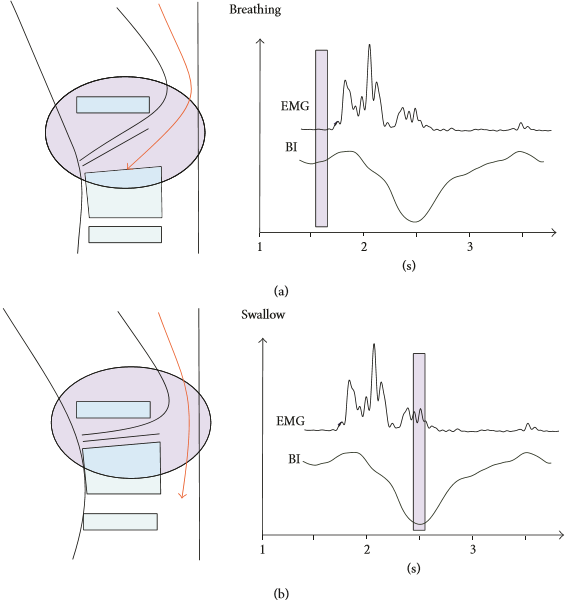
\includegraphics[width=7cm]
{Figure/EMGBIGraph}}
\caption{Illustration af, hvodan emg-og bioimpedans signaler opfører sig under vejrtrækning og mad/drikke indtagelse\cite{Schultheiss2014}}
\label{EMGBIGraph} 
\end{figure}

\section{Problemformulering}

Dette projekt undersøger muligheden for at udvikle et device, der består af en bioimpedans sensor og en EMG-måler, der tilsammen kan monitorere og detektere synkefrekvensen hos raske personer. Devicet bliver fremover omtalt som synkerefleksmonitor(SRM). Dette Projekt vil søge svar til følgende spørgsmål: 

\begin{itemize}
\item Kan man udvikle en prisbillig bioimpedans sensor, der kan være alternativ til Fiber Endoskopisk Evaluering af Synkefunktionen (FEES) og Funktionel Videoradiologisk Evaluering af Synkefunktionen (FVES) til at undersøge synkefrekvensen på personer, der er ramt af dysfagi?
\item Kan man kombinere bioimpedans sensor og EMG-måler til måling af dysfagi ?


\end{itemize}
Ved hjælp af systematisk og ikke-systematisk litteratursøgning vil disse spørgsmål blive besvaret gennem dette projekt. 

\section{Formål}

Formålet med dette projekt er at udvikle et produkt, der består af en bioimpedans-måler(BI-måler), der kan måle pålidelige bioimpedans signaler, samt kombinere BI-måleren med en kommerciel EMG sensor for at kunne detektere synkefrekvensen på raske objekter. Det overordnet systemet, der vil blive realiseret består af en BI sensor med elektroder, som er koblet til et rask objekt, en EMG måler med tre elektroder, som også er koblet til det samme objekt og en pc som anvendes til processering og visning af data til et sundhedspersonale, se figur \ref{KonceptuelDiagram}.  

\begin{figure}[H]
\centering
{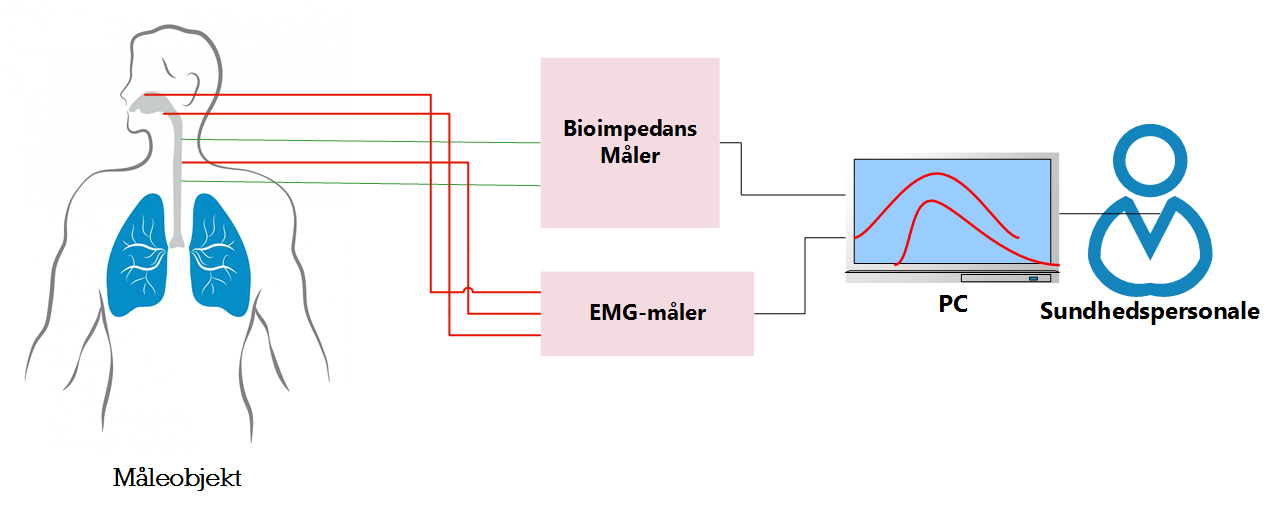
\includegraphics[width=11cm]
{Figure/KonceptuelDiagram}}
\caption{Illustration af  det overordnet system som dette projekt vil realisere}
\label{KonceptuelDiagram}
\end{figure}

Projektet vil fokusere på udvikling af den anbefalede prisbillige bioimpedans-måler(BI-måler). Det er ligeledes projektets mål at genskabe de to signaler, der er vist på figur \ref{EMGBIGraph}. EMG-måleren bruges som supplerende redskab til BI-måleren, da den kan detektere muskelaktiviteter, som finder sted før, under og efter et synk. Disse muskelaktiviteter er en forudsætning for at synkningen kan ske. 

Det skal dog for god ordens skyld understreges at systemet, der realiseres i dette projekt er på Proof-of-Concept stadie og må derfor ikke anvendes til klinisk brug. Det er ikke projektets mål at udvikle en endelig BI-måler, der kan sættes i produktion eller anvendes til screening af personer med mistanke for dysfagi. 

\section{Projektdeltagere og hovedansvarsområder} 
Arbejdsfordelingen i mellem gruppemedlemmerne er fordelt ligeligt på grund af gruppens størrelse. Gruppen har valgt at dele projektet op i en software-og hardwaredel, hvor alle i gruppen har ansvaret for  begge dele. Argumentet for denne kollektive ansvarsfordeling er valgt, da gruppens medlemmer har vurderet, at en skarp opdeling af ansvarsområder vil medføre mindre koordinering og risiko for, at man isolere sig kun til sit ansvarsområder. Tabel \ref{Ansvarsfordeling} viser den valgte ansvarsfordeling. 

\begin{table}[H]
\centering

\begin{tabular}{|l|l|}
\hline
\textbf{Projektdeltagere}        & \textbf{Hovedansvarsområder}  \\ \hline
Mohamed Hussein Mohamed & Hardware \& Software \\ \hline
Martin Banasik          & Hardware \& Software \\ \hline


\end{tabular}

\caption{indeholder gruppemedlemmernes navne og hovedansvarsområder }
\label{Ansvarsfordeling}
\end{table}


